\section{Methodology}
\label{sec:method}

The key idea in our approach is as follows.
Fix a point $x$ and let $\hat{m}_h(x)$ denote an estimator of $m(x)$ based on a vector of smoothing parameters $h=(h_1, \ldots, h_d)$. 
If $c$ is a scalar, then we write $h=c$ to mean $h=(c, \ldots, c)$.

Let $M(h)=\E(\hat{m}_h(x))$ denote the mean of $\hat{m}_h(x)$. 
For now, assume that $x=x_i$ is one of the observed data points and that $\hat{m}_0(x) = Y_i$.
In that case, $m(x) = M(0)=\E(Y_i)$. 
If $P=(h(t):\  0 \leq t \leq 1)$ is a smooth path through the set of smoothing parameters  with $h(0) = 0$ and $h(1) = 1$ (or any other fixed, large bandwidth) then
\begin{subequations}
    \begin{eqnarray}
        m(x) &=& M(0) = M(1) + M(0) - M(1) \\
        &=&  M(1) - \int_0^1 \frac{dM(h(s))}{ds} \, ds\\
        \label{eq::basic}
        &=&  M(1) - \int_0^1 \bigl\langle D(s), \overdot{h}(s)\bigr\rangle ds
    \end{eqnarray}
\end{subequations}
where
\begin{equation}
    D(h) = \nabla M(h) = 
    \left(\frac{\partial M}{\partial h_1},\ldots ,
        \frac{\partial M}{\partial h_d} \right)^T
\end{equation}
is the gradient of $M(h)$ and $\overdot{h}(s) = \frac{dh(s)}{ds}$ is the derivative of $h(s)$ along the path. 
A biased, low variance estimator of $m(x)$ is $\hat{m}_1(x)$.
An unbiased estimator of $D(h)$ is
\begin{equation}\label{eq::Z}
    Z(h) = \left(\frac{\partial\hat{m}_h(x)}{\partial h_1}, \ldots,
            \frac{\partial\hat{m}_h(x)}{\partial h_d} \right)^T.
\end{equation}
The naive estimator
\begin{equation}
    \hat{m}(x)=\hat{m}_1(x) -  \int_0^1 \bigl\langle Z(s), \overdot{h}(s)\bigr\rangle ds
\end{equation}
is identically equal to $\hat{m}_0(x)=Y_i$, which has poor risk since the variance of $Z(h)$ is large for small $h$. 
However, our sparsity assumption on $m$ suggests that there should be paths for which $D(h)$ is also sparse.
Along such a path, we replace $Z(h)$ with an estimator $\hat{D}(h)$ that makes use of the sparsity assumption.
Our estimate of $m(x)$ is then
\begin{equation}
\tilde{m}(x)  =  \hat{m}_1(x) - \int_0^1 \bigl\langle \hat{D}(s), \overdot{h}(s)\bigr\rangle ds\,.
\end{equation}
To implement this idea we need to do two things:
(i) we need to find a path for which the derivative is sparse and (ii) we need to take advantage of this sparseness when estimating $D$ along that path. 

\begin{figure}[t]
    \vskip5pt
    \psset{xunit=.5cm,yunit=.4cm}
    \pspicture(-6,0)(14,16)
    \psline[linewidth=1pt]{->}(2,2)(2,14)
    \psline[linewidth=1pt]{->}(2,2)(15,2)
    \psline[linewidth=1.5pt,linestyle=dashed]{->}(14,14)(14,3.2)
    \psline[linewidth=1.5pt]{->}(14,14)(13,14)(13,12)(12,12)(12,11)(12,6)(11,6)(10,6)(10,3.2)
    \psdot[dotsize=4pt](14,3)
    \psdot[dotsize=4pt](14,14)
    \psdot[dotsize=4pt](10,3)
    \rput(16,2){$h_2$}
    \rput(2,15){$h_1$}
    \rput(14.5,15.0){Start}
    \rput[l](17,3){Optimal bandwidth}
    \psline[linewidth=1.5pt]{->}(16.5,3)(14.3,3)
    \rput[l](14.5,8){Ideal path}
    \rput(9,8){Rodeo path}
    \endpspicture
    \vskip-10pt
    % \caption{Conceptual illustration: The bandwidths for the relevant variables ($h_1$) are shrunk, while the bandwidths for the irrelevant variables ($h_2$) are kept relatively large.}
    \caption{Conceptual illustration. The bandwidths for the relevant variables ($h_1$) are shrunk, while the bandwidths for the irrelevant variables ($h_2$) are kept relatively large. The simplest rodeo algorithm shrinks the bandwidths in discrete steps $1, \beta, \beta^2, \dots$ for some $0 < \beta < 1$.}
    \vskip10pt
    \label{fig:artwork}
\end{figure}


\section{Algorithm}
\label{sec:alg}

In this section, we show the detailed density rodeo algorithm for kernel density estimator which are known to be simple and have good properties. 
Assuming $x$ is a $d$-dimensional target point at which we want to evaluate the density values, let $\hat{f}_H(x)$ represents the kernel density estimator of $f(x)$ with a bandwidth matrix $H$. 
For a speciflc point, kernel density estimators smooth out the contribution of each observed data point over a local neighborhood of that data point. 
Assuming that $\mathcal{K}$ is a standard symmetric kernel, s.t. $\int \mathcal{K} (u) du = 1$,$\int u\mathcal{K} (u) du = 0_d$ while $\mathcal{K}_H(\cdot) = \frac{1}{det(H)} \mathcal{K}(H^{-1}\cdot)$ represents the kernel with bandwidth matrix $H = diag(h_1, \dots, h_d)$. 
\begin{equation}
    \hat{f}_{H}(x)=\frac{1}{n \operatorname{det}(H)} \sum_{i=1}^{n} \mathcal{K}\left(H^{-1}\left(x-X_{i}\right)\right)
\end{equation}

For the following density Rodeo algorithm, we assume that $\mathcal{K}$ is a product kernel and $H$ to be diagonal with elements $h = (h_1, \dots, h_d)$, therefore
\begin{equation}
    \begin{split} 
        Z_{j} 
        & =\frac{\partial \hat{f}_{H}(x)}{\partial h_{j}} \\ 
        &=\frac{1}{n} \sum_{i=1}^{n} \frac{\dot{K}\left(\frac{x_{j}-X_{i j}}{h_{j}}\right)}{K\left(\frac{x_{j}-X_{i j}}{h_{j}}\right)} \prod_{k=1}^{d} K\left(\frac{x_{k}-X_{i k}}{h_{k}}\right) \\ 
        & \equiv \frac{1}{n} \sum_{i=1}^{n} Z_{j i} 
    \end{split}
\end{equation}

For the variance term, since 
\begin{equation}
    \label{eq:sj}
    s_{j}^{2}=\operatorname{Var}\left(Z_{j}\right)=\operatorname{Var}\left(\frac{1}{n} \sum_{i=1}^{n} Z_{j i}\right)=\frac{1}{n} \operatorname{Var}\left(Z_{j 1}\right)
\end{equation}
Here, we used the sample variance of the $Z_{ji}$ to estimate $Var(Z_{j1})$. 
Therefore, for a Gaussian kernel, we have that
\begin{equation}
    \label{eq:zj}
    \begin{split} 
        Z_{j} 
        &=\frac{\partial \hat{f}_{H}(x)}{\partial h_{j}} \\ 
        &=\frac{1}{n h_{j}^{3}} \prod_{k=1}^{d} \frac{1}{h_{k}} \sum_{i=1}^{n}\left(\left(x_{j}-X_{i j}\right)^{2}-h_{j}^{2}\right) \prod_{k=1}^{d} K\left(\frac{x_{k}-X_{i k}}{h_{k}}\right) \\ 
        & \propto \frac{1}{n} \sum_{i=1}^{n}\left(\left(x_{j}-X_{i j}\right)^{2}-h_{j}^{2}\right) \prod_{k=1}^{d} K\left(\frac{x_{k}-X_{i k}}{h_{k}}\right) \\ 
        &=\frac{1}{n} \sum_{i=1}^{n}\left(\left(x_{j}-X_{i j}\right)^{2}-h_{j}^{2}\right) \exp \left(-\sum_{k=1}^{d} \frac{\left(x_{k}-X_{i k}\right)^{2}}{2 h_{k}^{2}}\right) 
    \end{split}
\end{equation}
Further, for a general kernel, we have
\begin{equation}
    Z_{j} 
    = \frac{\partial \hat{f}(x)}{\partial h_{j}}
    = - \frac{1}{n} \sum_{i=1}^{n}\left(\frac{1}{h_{j}}+\frac{x_{j}-X_{i j}}{h_{j}^{2}} \frac{d \log K}{d x}\left(\frac{x_{j}-X_{i j}}{h_{j}}\right)\right) \prod_{k=1}^{d} \frac{1}{h_{k}} K\left(\frac{x_{k}-X_{i k}}{h_{k}}\right)
\end{equation}

\begin{table}[ht]
    {\it Rodeo: Hard thresholding version}
    \vskip5pt
    \hrule
    \vskip5pt
    \begin{enumerate}
        \item {\it Select\/} $\beta_n = n^{-\alpha/\log^3 n}$ for some $0 < \alpha < 1$ and initial bandwidth
        \begin{equation}
            \label{eq:initial_h}
            \LL = \frac{c_0}{\log \log n}
        \end{equation}
        for some constant $c_0$.  
        Let $c_n$ be a sequence satisfying $c_n = O(1)$. 
        \item {\it Initialize\/} the bandwidths, and activate all covariates:
        \begin{enumerate}
            \item $h_j = \LL$, $j=1,2,\ldots, d$.
            \item $\A = \{1,2,\ldots, d\}$
        \end{enumerate}
        \item {\it While $\A$ is nonempty}, do for each $j\in \A$:
        \begin{enumerate}
            \item Compute the estimated derivative expectation: $Z_j$ (Eq. \ref{eq:zj})
            and $s_j$ (Eq. \ref{eq:sj}). 
            \item Compute the threshold
            $ \lambda_j = \displaystyle s_j \sqrt{2 \log (n c_n)}$.
            \item If $|Z_j| > \lambda_j$, then set $h_j \leftarrow \beta h_j$;
            otherwise remove $j$ from $\A$.
        \end{enumerate}
        \item {\it Output} bandwidths $h^\star=(h_1,\ldots,h_d)$ and estimator
        $\tilde{m}(x) = \hat{m}_{h^\star}(x)$.
    \end{enumerate}
    \vskip10pt
    \hrule
    \vskip10pt
    \caption{The hard thresholding version of the rodeo, which can be applied
    using the derivatives $Z_j$ of any nonparametric smoother.}
    \label{fig::hard-rodeo}
    \vskip15pt
\end{table}

\section{Theoretical Results}
\label{sec:theorem}

\begin{theorem}
    Under some moderate conditions, for every $\epsilon>0$ the number of iterations $T_n$ until the Rodeo stops satisfles
    \begin{equation}
        \mathbf{P}\left(\frac{1}{4+r} \log _{1 / \beta}\left(n^{1-\epsilon} a_{n}\right) \leq T_{n} \leq \frac{1}{4+r} \log _{1 / \beta}\left(n^{1+\epsilon} b_{n}\right)\right) \longrightarrow 1
    \end{equation}
    More over, the algorithm outputs bandwidths $h^*$ that satisfy
    \begin{equation}
        \mathbf{P}\left(h_{j}^{*}=h_{j}^{(0)} \text { for all } j>r\right) \longrightarrow 1.
    \end{equation}
    Also, we have
    \begin{equation}
        \mathbf{P}\left(h_{j}^{(0)}\left(n b_{n}\right)^{-1 /(4+r)-\epsilon} \leq h_{j}^{*} \leq h_{j}^{(0)}\left(n a_{n}\right)^{-1 /(4+r)+\epsilon} \text { for all } j \leq r\right) \longrightarrow 1
    \end{equation}
\end{theorem}

\begin{theorem}
    Under the same condition of theorem 1, the risk Rh⁄ of the density Rodeo estimator satisfles
    \begin{equation}
        \mathcal{R}_{h^{*}}=\tilde{O}_{P}\left(n^{-4 /(4+r)+\epsilon}\right)
    \end{equation}
    for every $\epsilon>0$.
\end{theorem}

These theoretical properties show that rodeo algorithm guarantees convergence within a finite step in probability, outputs $h^*$ will converge to its true value in probability and the risk of density Rodeo estimator is of order $n^{-4/(4+r)+\epsilon}$ which is the optimal order we can expect. 

\section{Simulation}
\label{sec:sim}

In this section, we applied the density rodeo on both synthetic and real data, including onedimensional, two-dimensionalexamples to investigate how the density estimation rodeo performs in various conditions. 
For the purpose of evaluating the algorithm performance quantitatively, we need some criterion to measure the distance between the estimated density function with the true density function. 

In the following, we first use the simulated data, about which we have known the true distribution function, to investigate the algorithm performance. 
% Then our algorithm is also applied on some real data for analysis and compare our results with the results gotten from the other authors. 

\subsection{One-dimensional examples}
First, we illustrate the performance of the density Rodeo algorithm in one dimensional examples. 
We have conducted a series of comparative study on a list of 15 ``test densities'' proposed by \cite{marron1992exact}, which are all normal mixtures representing many difierent types of challenges to density estimation. Our method achieves a comparable performance as the kernel density estimation with bandwidth selected by unbiased cross-validation (from the base library of R ). 
Due to the space consideration, only the strongly skewed example is reported here, since it demonstrates the advantage of adaptive bandwidth selection for the density rodeo algorithms. 

\begin{example}[Strongly skewed density]
    This density is chosen to resemble to lognormal distribution, it distributes as 
    \begin{equation}
        X \sim \sum_{i=0}^{7} \frac{1}{8} \mathcal{N}\left(3\left(\left(\frac{2}{3}\right)^{i}-1\right),\left(\frac{2}{3}\right)^{2 i}\right)
    \end{equation}
\end{example}
$200$ samples were generated from this distribution, The estimated density functions by the density rodeo algorithm, the density rodeo algorithm, and kernel density estimator with bandwidth chosen by unbiased cross validation are shown in Figure~\ref{fig: 1d rodeo 4in1}. 
In which, the solid line is the true density function, the dashed line illustrates the estimated densities by difierent methods. 
The density rodeo works the best, this is because because the true density function is strongly skewed, the flxed bandwidth density estimator can not flt the smooth tail very well. 
The last subplot from Figure~\ref{fig: 1d rodeo 4in1} illustrates the selected bandwidth for the density rodeo method, it shows how smaller bandwidths are selected where the function is more rapidly varying. 
The plots show that the density rodeo works better than the remaining two methods, while the rodeo and the unbiased cross-validation methods are comparable in this one dimensional example. 

\begin{figure}[t]
 \centering
 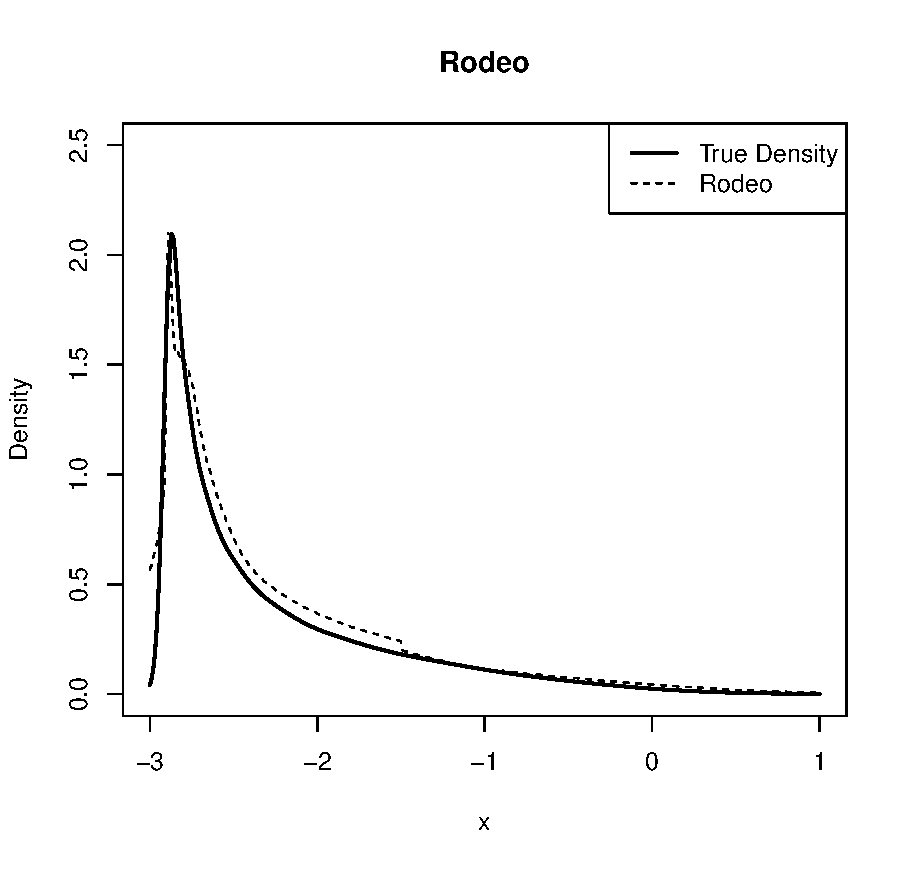
\includegraphics[width=0.7\textwidth]{pic/pic1.pdf}
 \caption{Local kernel density Rodeo.}
 \label{fig:1d rodeo 1}
\end{figure}

\begin{figure}[ht]
    \centering
    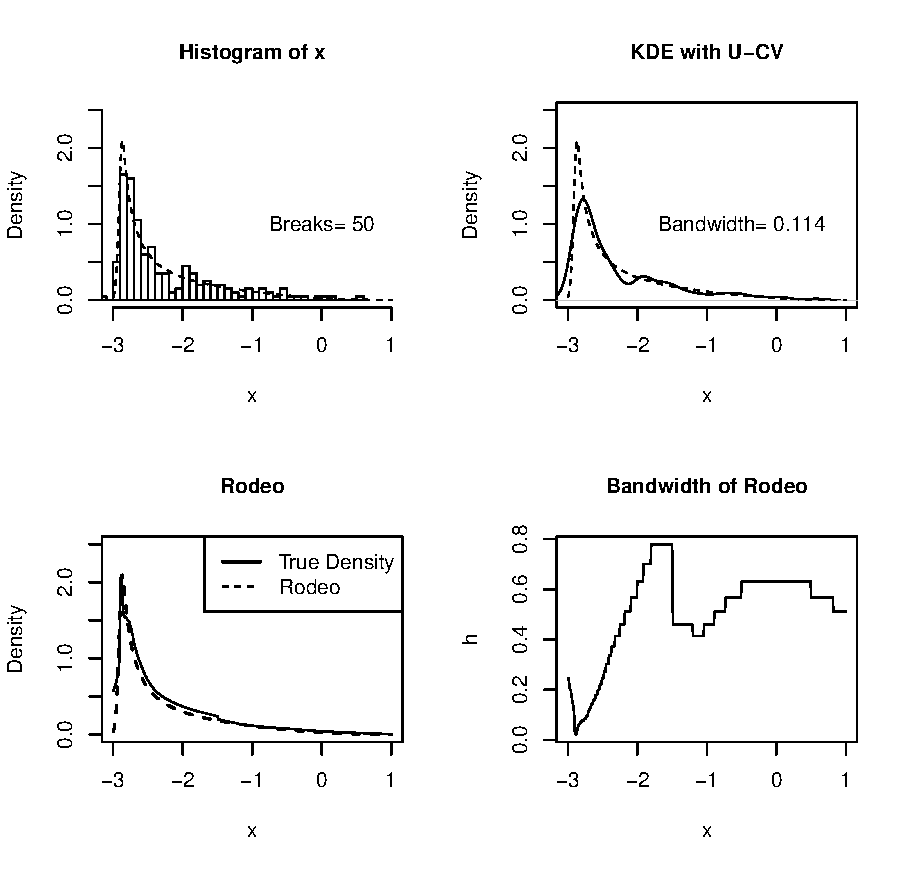
\includegraphics[width=1\textwidth]{pic/pic2.pdf}
    \caption{The difierent versions of the algorithms run on the highly skewed unimodal example. The first three plots are results for the difierent estimators, the last one is the fitted bandwidth for the density rodeo algorithm.}
    \label{fig: 1d rodeo 4in1}
\end{figure}

In stead of showing the positive cases where the density rodeo works well, we also give out a negative example. 
Which is a combined Beta distribution from \cite{loader1996local}.

\begin{example}[Combined Beta density]
    The density function is a Beta mixtures on the support of [0, 1], it has a strong boundary efiect on the left side, the density function is 
    \begin{equation}
        \begin{split}
            f(x) 
            & = \frac{2}{3} Beta(1,2) + \frac{1}{3} Beta(10, 10) \\
            & = \frac{2}{3} 2(1-x) + \frac{1}{3} \frac{19 !}{9 !^{2}} x^{9}(1-x)^{9} \\
        \end{split}
    \end{equation}
    altogether 500 samples were generated from this distribution, the estimated density functions by difierent methods are shown in Figure~\ref{fig: 1d rodeo 4in1 2}. 
\end{example}

\begin{figure}[ht]
    \centering
    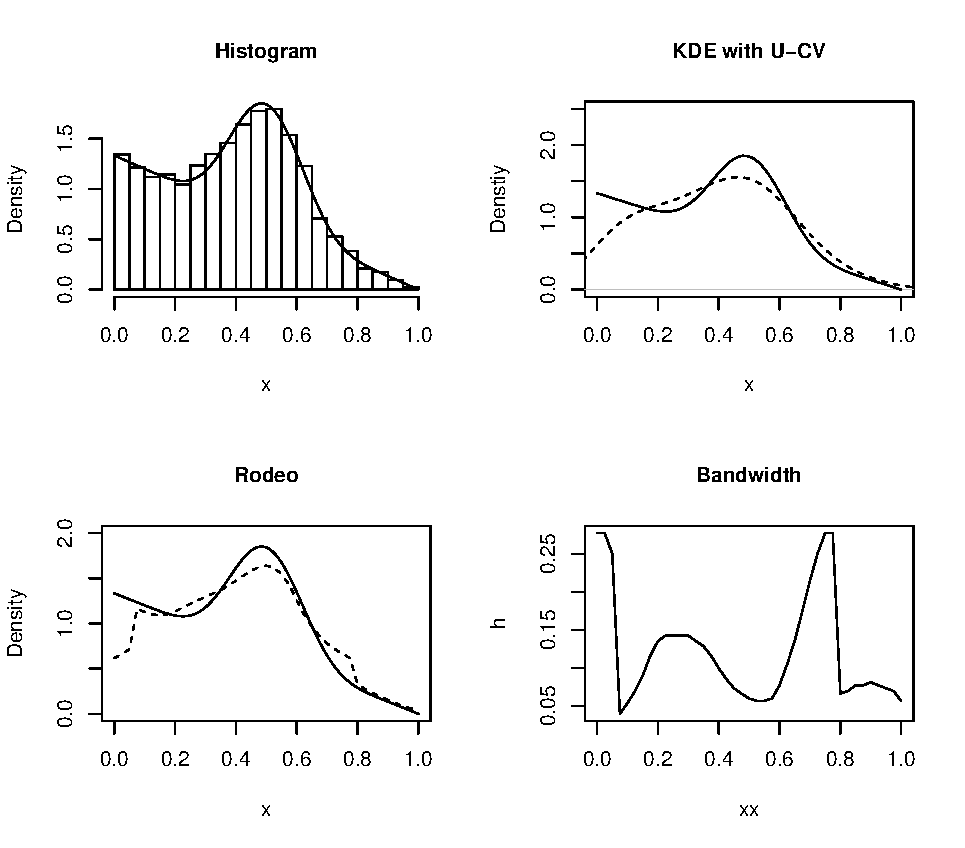
\includegraphics[width=\textwidth]{pic/pic3.pdf}
    \caption{Results for the combined beta distribution. The first three plots are results for difierent estimators, the last one is the fitted bandwidth for the local density rodeo algorithm. In the first three plots, the solid lines represent true density functions and the dash lines represent different estimators respectively.}
    \label{fig: 1d rodeo 4in1 2}
\end{figure}

Similar as before, the solid line is the true density function, while the dashed line illustrates the estimated functions. 
In this case, the rodeo and the unbiased cross-validation estimate the density function well. 
However, the rodeo fails to flt the right tail. 
From the bandwidth plot (as shown in the last subplot in Figure~\ref{fig: 1d rodeo 4in1 2}), we see that the rodeo tends to select larger bandwidth near the right boundary, which cause the problem. 

From the estimated bandwidth plot, we see that the boundary efiect problem is alleviated. 

\subsection{Two dimensional example}
Here, two 2-dimensional examples are showed due to its ease of illustration. 
One example used a synthetic dataset, the other one uses some real data analyzed by the other authors. 
The density rodeo’s performance is compared with a built-in method named KDE2d ( from MASS package in R ). 
The empirical results show that the density rodeo algorithm works better than the built-in method on the synthetic data, where we know the ground truth. 
For the real-world dataset, where we do not know the underling distribution, our method achieves a very similar result as those of the original authors who analyzed this data before. 
\begin{example}[Beta distribution with irrelevant unifrom distribution]
    \begin{equation}
        \begin{split}
            X_{1} & \sim \frac{2}{3} \operatorname{Beta}(1,2)+\frac{1}{3} \operatorname{Beta}(10,10) \\ 
            X_{2} & \sim \text {Uniform} (0,1)
        \end{split}
    \end{equation}
\end{example}

\begin{figure}[ht]
    % \centering
    \hspace{-6em}
    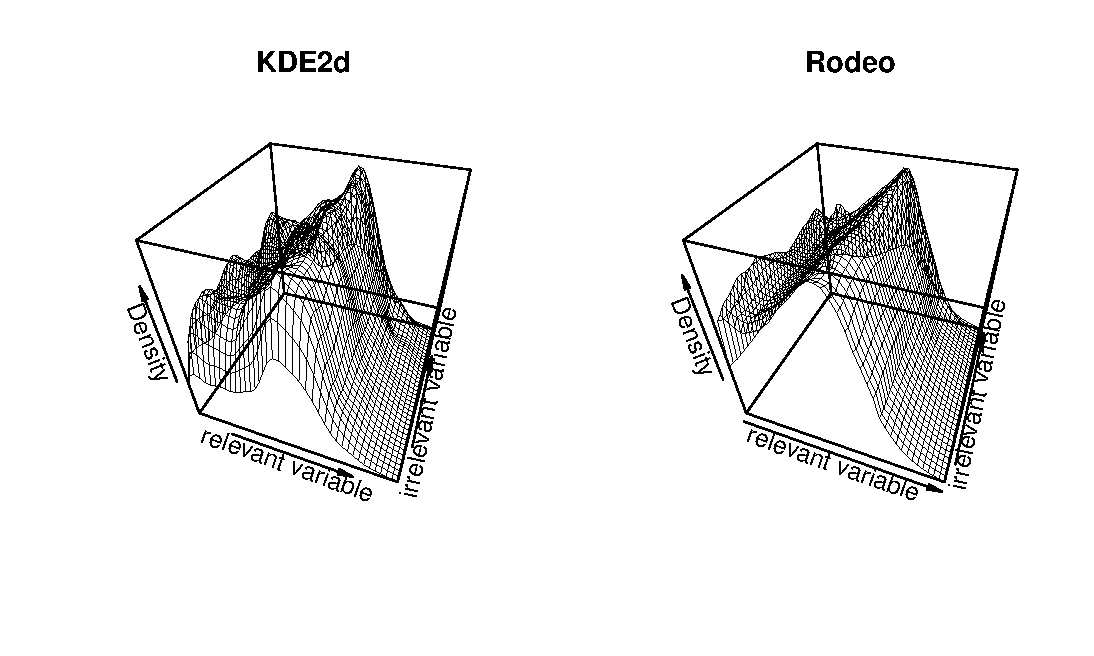
\includegraphics[width=1.2\textwidth]{pic/pic5.pdf}
    \caption{Results for the combined beta distribution. The first three plots are results for difierent estimators, the last one is the fitted bandwidth for the local density rodeo algorithm. In the first three plots, the solid lines represent true density functions and the dash lines represent different estimators respectively.}
    \label{fig: 2d rodeo 2in1}
\end{figure}

Figure~\ref{fig: 2d rodeo 2in1} illustrates the estimated density functions by the density rodeo and the built-in method KDE2d. 
From which, we see that the rodeo algorithm flts the irrelevant uniform dimension perfectly, while KDE2d fails. 
For a quantitative comparison, we evaluated the empirical Hellinger distance between the estimated density and the true density, the rodeo algorithm outperforms KDE2d uniformly on this example. 
For a qualitative study, Figure~\ref{fig: 2d rodeo 2in1} illustrates the numerically integrated marginal distributions of the two estimators (not normalized), it’s consistent with the previous observations. 

Further, we can apply this algorithm on high dimensional data ($d \ge 3$) with spare true variables, but we lack of time and computation resource to adjust the parameters and get proper results. 


\section{Conclusion}
\label{sec:conclusion}
This work is mainly purposed to illustrate the generality of the rodeo framework \citep{Lafferty2005, wasserman2006rodeo, Lafferty2008}. 
Under some suitably-deflned sparsity conditions, the previously developed nonparametric regression framework is easily adapted to perform high-dimensional density estimation. The resulting method is both computationally e–cient and theoretically soundable. Empirical results show that our method is better than the built-in methods in some cases. 

In the future, we can try to develop rodeo using paralleled or distributed computation to speed it up further. Also we can expend its variation for example boostrap sampling,  using soft threshold to select $h$, backward method or any other statistical method.